
\chapter{丘奇、图灵、塔斯基及别的人}

\section{形式的和非形式的系统}

现在可以展开本书的一个主要论题了,那就是:思维的每一个方面,都可以看成是从较高的层次上描述的一个位于较低层、受某些简单的乃至形式的规则支配的系统。当然,这个“系统”就是大脑——除非谈论的是在另一种媒质(比如一台计算机的电路)中流动的思维过程。形象地说,这是一个支撑着“非形式系统”的形式系统,那个非形式系统能一语双关、能发现数字中的模式、会忘记人的姓名、会走臭棋、等等。我们从外部看到的是它的非形式化的、公开的、软件的层次。作为对照,它还有一个形式化的、隐蔽的、硬件的层次(或叫“基质”),这是一部令人望而生畏的机器,它根据物理地嵌入其中的某些确定的规则以及与之密切相联的信号输入,在各个状态之间进行转换。

像这样一种对大脑的看法,肯定会有很多哲学的和其它方面的推论。我打算在这一章里详细地说明这样一些推论。其中之一是说,这种看法似乎蕴涵着:从本质上讲,大脑是某种“数学”对象。其实,这充其量也不过是看待大脑的一种十分笨拙的办法。因为即便在技术意义或抽象意义上说大脑是某种类型的形式系统,仍然无法摆脱下面的事实:数学家只与那些简单的、考究的形式系统打交道,在那些系统中,一切东西都有着极为清晰的定义。而大脑则与此大相径庭,它的上百亿个不完全独立的神经元彼此是近乎随机地相联接的。所以,数学家决不会去研究实际的大脑网络。如果你把“数学”定义为数学家喜欢作的事情,那么大脑的性质就不是数学性质了。

要想了解像大脑这样的复杂系统,唯一的方法是在越来越高的层次上对之组块,因而每一步都要损失一些严格性。出现在最顶层上的,是一个“非形式系统”,它要服从许多复杂到我们找不到合适的词汇去思考的规律。而这正是人工智能的研究所想找到的东西。它具有与数学研究大不相同的味道。尽管如此,还是与数学有个松散的联系:从事人工智能研究的人,通常都有很强的数学背景,并且,数学家有时也会对自己大脑的工作感兴趣。下面这段引自斯坦尼斯拉夫·乌兰姆的自传《一位数学家的奇遇》的文字,正好说明了这一点。

\begin{quote}
依我看,在揭示……联想的本质时,有了计算机提供的实验手段,就可以做更多的事情了。这种研究必定要把概念、符号、符号组成的类、类组成的类等等进行分级,就像在研究数学和物理结构的复杂性时所做的那样。

人脑的思维过程一定有某种窍门——某种递归公式。一组神经元能自动开始工作,有时用不着外来剌激,而是靠一个具有递增模式的迭代过程。它在大脑中游来荡去,而且,它的发生方式必定依赖于对类似模式的记忆。\note{斯坦尼斯拉夫·乌兰姆,《一位数学家的奇遇》,第13页。}
\end{quote}

\section{直觉和值得赞美的螃蟹}

人工智能[Artificial Intelligence]常被简称为“AI”。如果要我来解释这两个字母的涵义,我会说它也可以被理解为“人工直觉”[Artificial Intuition]或“人工意象”[Artificial Imagery]。人工智能的目标是要弄清,当人的大脑在一种十分复杂的环境中不动声色地从大量可能性中选择哪一种最为合理时,会发生什么事。在现实生活的许多场合,演绎推理之所以不适用,并不是因为它会得出错误答案,而是因为它会得到过多的正确然而无关的断言。为了满足推理本身的充分性,需要同时考虑的东西也就太多了。请看这样一段很短的对话:

\begin{quote}
“那天,我从报上读到——”

“噢——你曾读报来着?那就可知你有眼睛。或者说至少有一只眼睛。或者更确切地说你那时至少有一只眼睛。”
\end{quote}

这就需要一种辨别的能力——“在这里,什么东西重要,什么不重要?”与此相关联的,是一种对简洁的感受力和对美的感受力。这些直觉是从哪来的呢?它们是怎样从作为基础的形式系统中显现出来的?

《的确该赞美螃蟹》里显示了螃蟹智慧的一些非凡力量。按他自己对这种力量的说法,他只不过是在听音乐,并区分优美的音乐和不优美的音乐(显然,他有一条明确的分界线)。然后,阿基里斯找到了另一种描述螃蟹能力的方法:螃蟹把数论陈述分为真的和假的两个范畴。可是螃蟹坚持说,如果他真的做到了这一点,那也纯属偶然,因为按照他自己所承认的,他在数学方面是无知的。然而更加使阿基里斯不解的是,螃蟹的行为看上去直接违背了阿基里斯所熟悉的一项备受称颂的元数学结果:

\begin{thm}{丘奇定理}
没有一个切实可靠的方法总能区分开TNT的定理和非定理。
\end{thm}
这是美国逻辑学家丘奇于1936年证明的。与此密切相关的是下面这个结果,我称之为

\begin{thm}{塔斯基—丘奇—图灵定理}
没有一种切实可靠的方法总能区分开真的数论语句和假的数论语句。
\end{thm}

\section{丘奇—图灵论题}

为了更好地理解\emph{丘奇定理}和\emph{塔斯基—丘奇—图灵定理},我们先得描述一下作为它们的基础的一种思想,那就是丘奇—图灵论题(通常也叫“丘奇论题”),因为丘奇—图灵论题确实是数学、大脑及思维的哲学中最重要的概念之一。

实际上,像泡茶一样,丘奇—图灵论题也能有各种不同的浓度。所以,我要以好几种形式来表述它,并且看看这些不同的形式各自蕴涵着什么。

第一种形式听起来十分幼稚——事实上几乎是空洞无物:

\begin{thm}[2\ccwd]{丘奇—图灵论题,同义反复形式}
数学问题只能通过数学推演来解决。
\end{thm}

自然,整体的意义寓于作为组成成分的各术语的意义之中。所谓“数学问题”,我指的是判定某个数是否具有一个给定的算术性质。看得出,借助于哥德尔配数法和相应的编码手段,几乎每一个数学分支的每一个问题都能归入这种形式。所以,“数学问题”一词仍保持其通常含义。“数学推演”又怎么讲呢?当你试图确定一个数是否具有某种性质时,似乎只有一遍又一遍地结合使用很少量的几个运算——加法、乘法、验证相等与不等。这就是说,循环地使用这些运算,好像就是使我们得以深究数的世界的唯一工具。要注意“好像”这个词。这是有关丘奇—图灵论题的关键字眼。我们可以给出一个“修订本”:

\begin{thm}[2\ccwd]{丘奇—图灵论题,标准形式}
假设有一种方法,一个有感知能力的生物可以根据这种方法逐个把数分成两类。又假定这种方法总能在有穷时间内得出答案,而且对于给定的数,这种方法总给出相同的答案。那么:存在一个有终止的FlooP程序(即一般递归函数),它给出的答案恰好与这个有感知能力的生物的方法所得到的答案一样。
\end{thm}

中心假设说穿了就是:把数分成两类的任何一个心智过程都可以用FlooP程序来描述。直觉上的一个信念是,这种心智过程中没有使用什么超出了FlooP能力的工具,而且使用这些工具的方式也没有超出不限次数的迭代(FlooP允许这么做)。丘奇—图灵论题不是数学定理意义上的一个可证的事实——它是有关人脑中所使用的过程的一个假设。

\section{大众过程形式}

此刻,有些人可能会感到,丘奇—图灵论题的这种形式断定的东西太多。这些人可以提出如下的反对意见:“也许有像螃蟹这样的人——他对数学有着几乎是神奇的洞察力,但像其他人一样,他自己对这种特殊能力也一无所知——那么这种人的心智机制大概就能执行在FlooP中找不到对应物的运算。”这种想法就是说:或许我们会有一些下意识的潜力,可以做出超越意识过程的事情——这些事情大概无法用基本FlooP运算表示。对这些反对派,我们将给出该论题的一个弱形式,它在大众的和个人的心智过程之间作了区分。

\begin{thm}[2\ccwd]{丘奇—图灵论题,大众过程形式}
假设有一种方法,一个有感知能力的生物可以根据它逐个把数分成两类。又假设这种方法总能在有穷的时间内得出结果,并且对给定的数它总能给出相同的结果。同时,还要假定这种方法可以通过语言由一个有感知能力的生物不走样地传达给另一个有感知能力的生物。那么,存在一个有终止的FlooP程序(即一般递归函数),它给出的答案恰好和这个有感知能力的生物的方法所得到的答案一样。
\end{thm}

这就是说,大众接受的方法受“FlooP化过程”的管辖,但对个人特有的方法,它却什么也没断定。当然它并没有说个人特有的方法都是FlooP力所不及的,不过至少还是留有这样的余地。

\section{湿利尼吠萨·拉玛奴衍}

作为反驳任何一种强形式丘奇—图灵论题的证据,我们来看看二十世纪初叶著名的印度数学家湿利尼吠萨·拉玛奴衍(1887--1920)(\fig{105})这个实例。他出生于印度最南部的泰米尔邦,高中时学过一点数学。一天,一个认为拉玛奴衍有数学天分的人,介绍他看一本略为过时的分析教科书,拉玛奴衍立即狼吞虎咽起来。于是他开始突入分析世界,二十三岁前后,他就已作出了一些他认为值得花费时间的发现。他不知道该向谁求教。可不知怎么回事,有人就谈到了远在英国的一位数学教授——哈代。于是拉玛奴衍把他最好的一些结果全都装进一个纸袋,连同朋友们帮他用英文写的一封说明信一起,寄给事先毫不知情的哈代。下面这段话录自哈代对自己接到这包东西时的描述:

\begin{quote}
……一下子就能看出,拉玛奴衍一定还有很多更普遍的定理,肯定还藏着很多东西……\lnote{(有些公式)}完全使我折服了。以前我从未见过任何一种哪怕是稍许类似的东西。仅仅看一眼就足以说明只有最高水平的数学家才写得出来。它们必定是真的,因为假如它们不真,不可能会有人具备杜撰它们的想象力。最后……作者肯定百分之百地诚实,因为大数学家比具有如此难以置信的技巧的窃贼或骗子更常见。\note{詹姆斯·纽曼[James R.Neuman],“湿利尼吠萨·拉玛奴衍”,载詹姆斯·纽曼编,《数学世界》[\bn{The World of Mathematics}],纽约:Simon and Schuster,1956年版,第一卷,第372--373页。}
\end{quote}

\begin{figure}
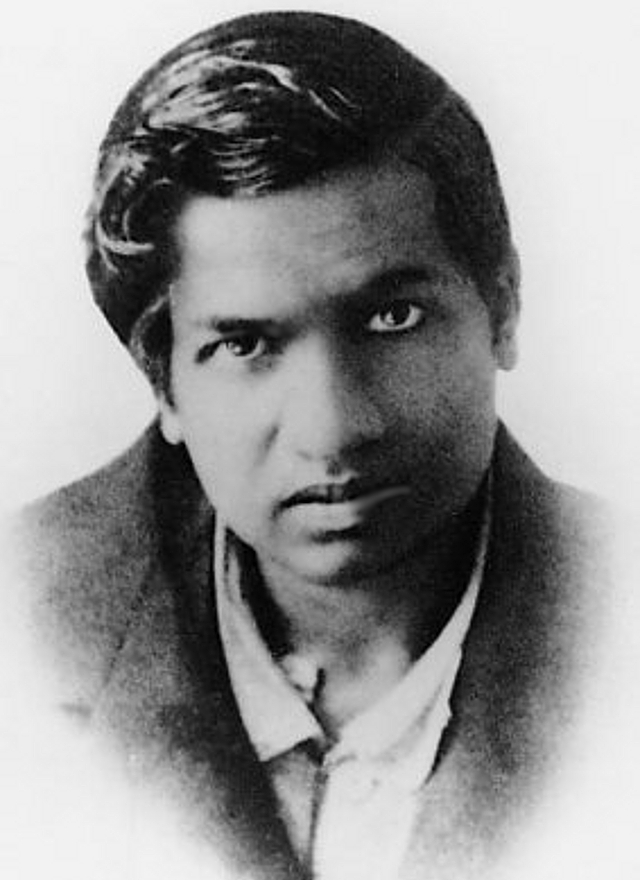
\includegraphics[width=.5\textwidth]{img_105.jpg}
\[
\cfrac1{
  1+\cfrac{\me^{-2\uppi\sqrt{5}}}{
    1+\cfrac{\me^{-4\uppi\sqrt{5}}}{
      1+\cfrac{\me^{-6\uppi\sqrt{5}}}{
        \rule{0pt}{\baselineskip}1+\raisebox{-.7\baselineskip}{$\ddots$}}}}}=
\Biggl(
\frac{\sqrt5}{1+\sqrt[5]{5^{3/4}\biggl(\dfrac{\sqrt{5}-1}2\biggr)^{5/2}-1}}
-\frac{\sqrt5+1}2
\Biggr)\me^{2\uppi/\sqrt{5}}
\]
\caption[湿利尼吠萨·拉玛奴衍及其神奇的印度旋律之一。]
  {湿利尼吠·拉玛奴衍及其神奇的印度旋律之一。}
\end{figure}

这次通信的结果是,拉玛奴衍根据哈代的建议,于1913年来到英国,随后就开始了一场以拉玛奴衍三十三岁早逝于肺结核为结局的紧张合作。

拉玛奴衍具有一些使他有别于大多数数学家的极不寻常的特点。其中之一是他缺乏严格性。他常常会简单地陈述一个结果,然后坚称这个结果完全来自自己模糊的直觉,这与那个有意识的进行研究探索的领域是格格不入的。事实上,他常说女神娜摩吉利在梦中给他灵感。这种情形一再发生。使之更加神秘——也许甚至是使之充满了神奇特性——的是,拉玛奴衍的这些“直觉定理”中有很多是错的。世上有一种奇怪的悖论效果:一件你认为不会促使人们轻信,而是会使易轻信的人变得开始怀疑的事情,实际上却具有相反的效果。因为它击中了轻信者心理上的弱点,用暗示人类本性中一些令人困惑的非理性侧面的办法吊起了他们的胃口。这就是拉玛奴衍出错时所发生的情形:很多受过教育的人,以一种强烈的倾慕之心,相信某些被看成拉玛奴衍的直觉能力的东西,认为它证明了有一种神奇的、洞察真理的力量存在,而他难免出错这一事实甚至可能是加强了——而不是削弱了——这种信念。

当然,没人否认拉玛奴衍来自印度最落后的地区。在那里,行乞化缘和其它一些古里古怪的印度习俗已经沿袭了数千年,而且还将继续下去,其频繁程度大概要超过高等数学课。拉玛奴衍的那些偶然的失误并没有提醒人们认清他只是个人,反倒自相矛盾地激起了一种想法:他的错误总有某种“更深刻的正确性”——某种西方人的心智或许不可企及的“东方的”正确性。这是多么诱人而且近乎无法抵御的想法啊!即便是哈代——他该是第一个否认拉玛奴衍有特异功能的人——在谈到拉玛奴衍的某次失败时也说:“从某种意义上说,我并不认为他的这次失败就不比任何一次成功更精彩。”

拉玛奴衍的数学个性中另一个突出的特点(照他的同事李特伍德的说法),就是“与整数的友谊”。相当多的数学家都在不同程度上具有这样的特点,而拉玛奴衍则登峰造极。有两则轶事可以说明他的这种特殊能力。第一则为哈代所讲:

\begin{quote}
记得有一次他生病住在普特涅,我去看他,乘的是一部号码为1729的出租马车,我注意到对这个数我翻不出什么花样,只希望它不是什么凶兆。“不”,他听后答道,“这是个很有意思的数:它是能用两种不同方法表示成两个数的立方和的最小的数。”自然,我就问他是否知道对应于四次方的这样一个问题的答案。他想了一会,回答说他一下子找不到例子,第一个这样的数一定很大。\note{詹姆斯·纽曼[James R.Neuman],“湿利尼吠萨·拉玛奴衍”,载詹姆斯·纽曼编,《数学世界》[\bn{The World of Mathematics}],纽约:Simon and Schuster,1956年版,第一卷,第375页。}
\end{quote}

实际上,对于四次方,答案是:
\[
635318657=134^4+133^4=158^4+59^4
\]
而关于二次方的类似问题则要容易的多,读者可以试着动手解一解,说不定会觉得很好玩的。

考虑一下哈代为什么会直接跳到四次方去,其实是很有意思的。因为毕竟是存在好几种合理而又自然的方式,能在不同的维度上推广方程
\[
u^3+v^3=x^3+y^3
\]

例如,把一个数用三种不同方法表示成两个立方之和的问题:
\[
r^3+s^3=u^3+v^3=x^3+y^3
\]
或者,可以用三个不同的立方数:
\[
u^3+v^3+w^3=x^3+y^3+z^3
\]
或者,甚至可以同时对所有的维度都推广:
\[
r^4+s^4+t^4=u^4+v^4+w^4=x^4+y^4+z^4
\]
即:“能用三种不同方法表示成三个数的四次方之和的最小数是什么?”不过,从某种意义上来说,哈代的推广是“大多数数学家所倾向的”。这样一种数学美学的意义最终能不能得以程序化呢?

另一则轶事出自拉玛奴衍的同胞拉戈那罕为他所写的传记,传记中称这件事为“拉玛奴衍的闪念”,那是拉玛奴衍在剑桥时代的印度朋友玛哈拉诺比斯博士讲述的。

\begin{quote}
又有一次,我去他家吃午饭,当时第一次世界大战已经打了一些时候了。我手里拿着一份《海滨杂志》月刊,当时这家杂志常发表一些谜题供读者解答。拉玛奴衍正把锅坐在火上,在里面搅拌着什么东西准备午饭,我则坐在桌子旁边翻阅杂志。有一个涉及两个数之间的关系的问题吸引了我。问题的细节已经忘了,不过我还记得它的类型。是说两名英国军官住在巴黎一条长街上的两所房子里,其门牌号码有某种特殊的联系,问题就是:求出这两个数。题目并不难,我通过尝试、订正,花了几分钟就解出来了。
\begin{dialogue}[topsep=\medskipamount]
\item[玛哈拉诺比斯]\dlnote{(开玩笑地)}有个问题你。
\item[拉玛奴衍]什么问题?说吧。\dlnote{(他继续在锅里搅着。)}
\end{dialogue}

我把《海滨杂志》上的问题读了一遍。

\begin{dialogue}[topsep=\medskipamount]
\item[拉玛奴衍]请把答案记下来。\dlnote{(他念出一个连分数。)}
\end{dialogue}

连分数的第一项是我已经得到的解,而如果街上的门牌号数可以无限制地增长下去的话,后续各项就将依次成为这个问题的后续的解。我感到十分惊奇。

\begin{dialogue}[topsep=\medskipamount]
\item[玛拉哈诺比斯]你一眨眼之间就得到这个解了吗?
\item[拉玛奴衍]我一听到这个问题就明显感到,解显然是一个连分数,于是我就想:“是个什么样的连分数呢?”然后答案就在我脑子里出现了。就是这么简单。\note{拉戈纳罕[S.R.Ranganathan],《拉玛奴衍》,第81--82页。}
\end{dialogue}
\end{quote}

拉玛奴衍逝世之后,常有人向他的最密切的合作者哈代问起,拉玛奴衍的思维方式是否有什么超自然的或异国情调的奇异因素。哈代作了如下的评述:

\begin{quote}
我曾不时地被人问起:拉玛奴衍是否有什么特殊的奥秘?他的方法是否与其他数学家有实质上的不同?他的思维方式是否确实有什么不正规的东西?我无法以任何自信的或有说服力的方式来回答这些问题,不过我并不相信那些假设。我的信念是,从本质上讲,所有的数学家都在用同一性质的方法思维,拉玛奴衍也不例外。\note{詹姆斯·纽曼[James R.Neuman],“湿利尼吠萨·拉玛奴衍”,载詹姆斯·纽曼编,《数学世界》[\bn{The World of Mathematics}],纽约:Simon and Schuster,1956年版,第一卷,第375页。}
\end{quote}

哈代在这里其实是在陈述他自己对丘奇—图灵论题的一种说法。我来发挥一下,就是:

\begin{thm}[2\ccwd]{丘奇—图灵论题,哈代形式}
从本质上讲,所有的数学家都同构。
\end{thm}
这还没有把每个数学家的数学潜力都等同于一般递归函数的潜力。要想做到这一点,你所需要做的事情也就是设法说明某个数学家的心智能力与递归函数的能力是一样的。这样,如果你相信丘奇—图灵论题的哈代形式,那就可以知道全体数学家都是如此了。

此后,哈代将拉玛奴衍和一些计算奇才作了比较:

\begin{quote}
他的记忆力和计算能力很不寻常,不过也不能说它们“反常”。当他需要做两个大数的乘法时,他是用普通的方法,只是他可以用不同寻常的速度和准确度来做好它,但也并不比任何一名天生迅速而又有计算习惯的数学家更快。\note{詹姆斯·纽曼[James R.Neuman],“湿利尼吠萨·拉玛奴衍”,载詹姆斯·纽曼编,《数学世界》[\bn{The World of Mathematics}],纽约:Simon and Schuster,1956年版,第一卷,第375页。}
\end{quote}
哈代描述了他所发现的拉玛奴衍突出的智力特征:

\begin{quote}
由于他的记忆、耐心和计算才能,他把综合能力、对形式的感觉能力和对假设的快速修订能力结合了起来,这经常出人意料,并使他在那个时代中自己的那个领域内无可匹敌。\note{詹姆斯·纽曼[James R.Neuman],“湿利尼吠萨·拉玛奴衍”,载詹姆斯·纽曼编,《数学世界》[\bn{The World of Mathematics}],纽约:Simon and Schuster,1956年版,第一卷,第375--376页。}
\end{quote}
这段文字中提到的那几种能力,依我看是对一般智能的某些最微妙的特征的精彩刻划。最后哈代颇怀眷恋地总结说:

\begin{quote}
\lnote{(他的工作)}没有最伟大的工作所必须具备的那种简洁性和必然性。如果不那么古怪,它就会更伟大一些。他的工作具有一种不可否认的天赋——意义深刻和无往不胜的独创性。如果他早在青年时代就被发现并受到一些训练,他就可能成为一名伟大的数学家,他就会完成更多新的、而且无疑是极为重要的发现。另一方面,那也将使他变得不那么像拉玛奴衍,而更像一名欧洲教授。这也许是得不偿失的。\note{詹姆斯·纽曼[James R.Neuman],“湿利尼吠萨·拉玛奴衍”,载詹姆斯·纽曼编,《数学世界》[\bn{The World of Mathematics}],纽约:Simon and Schuster,1956年版,第一卷,第376页。}
\end{quote}

哈代在说起拉玛奴衍时所用的浪漫方式,充分表达了他对拉玛奴衍的珍重。

\section{“心算家”}

还有一类人,他们的数学能力似乎得不到合理的解释——那就是所谓“心算家”,这些人能在心中(或别的什么地方)一眨眼之间完成复杂的计算。生于1824年,卒于1861年,并为欧洲的好几个政府雇来作计算工作的戴斯就是一个突出的例子。他不仅能心算两个一百位数的乘法,而且有一种不可思议的数量感。也就是说,他可以不用数数就“分辨出”一块地里有多少只羊或者一个句子里有多少个词等等,可以多到$30$个左右——这和我们大多数人显著不同,我们的这种感觉只在$6$个以内时才是可信的。

我不打算描述很多这类让人眼花缭乱的、但却有案可稽的“瞬息计算者”,因为这不是我此处的目的。不过我觉得,消除那种认为他们是用某种神秘的、不可分析的方法计算的想法,是重要的。尽管实际情况常常是:这种奇才的计算能力远远超过他们解释自己的结果的能力,不过偶尔也会出现一个具有其它智力天赋,同时也具有这种惊人的数字能力的人。根据这些人的自省以及广泛的心理学研究已经弄清:在瞬息计算者进行运算的过程中,并没有发生什么超自然的事情,而只是他们的心智非常自信地加速越过了各个中间步骤,就像天生的运动员迅速完美地从事一项复杂运动时那样。他们不是依赖某种顿悟般的瞬息闪念来得到答案(尽管在主观上他们当中有些人似乎感到是这么一回事),而是——像我们这些人一样——由一系列计算得到的,也就是说用FlooP(或BlooP)之类的过程得到的。

此外,能够说明并不存在什么“通往上帝的热线”的一条最明显的线索,是一个简单的事实:当用到的数字变大时,答案就出来得慢。可以设想,如果是上帝或“神谕”在提供答案,那么当数字变大时就不该变慢。人们也许可以找到一个更好的解释,说明瞬息计算所花的时间是如何随用到的数字的大小及用到的运算种类而变化的,并由此来推定所用的算法的某些特征。

\section{丘奇—图灵论题的同构形式}

这最终把我们带到加强了的丘奇—图灵论题标准形式:

\begin{thm}[2\ccwd]{丘奇—图灵论题,同构形式}
假定有一种方法,一个有感知能力的生物可以利用它逐个把数分成两类。又假定这种方法总能在有穷的时间内得到答案,而且对于一个给定的数总是给出相同的答案。那么,存在某个有终止的FlooP程序(即一般递归函数),它给出的答案恰好与这个有感知能力的生物的方法所得到的答案一样。而且,这个心智过程与这个FlooP程序在下述意义上同构:在某个层次上,计算机和大脑各自执行的那些步骤之间存在一个对应。
\end{thm}
应当注意,在这里,不仅结论加强了,而且也抹去了吞吞吐吐的大众过程形式中的那个有关通迅的附加条件。这个大胆的形式正是我们现在所要讨论的。

简而言之,丘奇—图灵论题的这种形式断言:当一个人计算某个问题时,他的心智活动可以同构地在某个FlooP程序中得到反映。不过读者应该清楚,这并不意味着大脑实际上是按照一个用FlooP语言写下的、尽是些\inst{BEGIN}、\inst{END}、\inst{ABORT}之类的FlooP程序而运行的——完全不是。这只不过是说各个步骤之间的次序与FlooP程序中相应的次序完全相同,而且计算的逻辑结构也可以在FlooP程序中得到反映。

现在,为了弄清这一思想的含义,我们得在计算机以及大脑中区分出不同的层次,否则这就会被误认为是十足的胡说。很可能,在人的头脑中进行的这些计算步骤都处于最高层次,并从较低的层次上得到支持,因而最终被“硬件”所支持。所以如果我们说到同构,那就意味着我们心照不宣地做了一个假设,即能把最高层隔离开来,从而使我们得以脱离其它层次来讨论这里发生的事情,并能把这个顶层对应到FlooP。说得更严格一些,这个假定就是说:存在一些软件实体充当着种种数学思维的角色,它们以某些能够严格反映为FlooP的方法起着作用(见\fig{106})。使这些软件实体得以实现的东西,是第十一章、第十二章以及《前奏曲,蚂蚁赋格》中讨论过的整个基础结构。对大脑和计算机的较低层次(例如神经元和位)上的同构作用,则没下任何断言。

\begin{figure}
%\includegraphics{img_106.png}
\begin{tikzpicture}[semithick]
\matrix[column sep=10mm,row sep=10mm,every node/.style={%
  draw,align=center,font=\linespread{1}\selectfont,inner sep=2mm}]{
\node(A){计算机程序\\(高级语言)};
& & \node[rounded rectangle](B){人脑\\(符号层)};\\
& \node[rounded corners=2mm](C){自然数\\的空间};\\
};
\draw[dashed]
      (A) -- (B) node[midway,above]{同构};
\draw (A.south) -- (C.west) node[midway,left,yshift=-1mm]{同构}
      (B.south) -- (C.east) node[midway,right,yshift=-1mm]{同构};
\end{tikzpicture}
\caption[联系着自然数、计算机和人脑的同构关系。]
  {自然数的性质能在人类大脑和计算机程序中得到反映。这两个不同的描述因而能在一个适当的抽象层次上彼此对应。}
\end{figure}

如果不拘泥于字面,丘奇—图灵论题的同构形式之所以能为人理解,是由于它说一个心算家在计算(比如说$\uppi$的对数)时所做的事情,同构于一部袖珍计算器在计算它时所做的事情。这里的同构是在算术步骤的层次上成立,而不是在更低的层次——神经元和集成电路之间——成立的。(当然,计算任何东西都可以有不同的方法,但不妨假定那部袖珍计算器——如果不提那个人——可以按任意特定的方式完成所要求的计算。)

\section{对关于现实世界的知识的表示}

当我们所考虑的范围是数论的时候,这件事看上去的确是合情合理的,因为此时发生各种事件的那个论域既小又清晰。而论域本身的边界、居民、法规也都是良定义的,就像用标准几何图形画出的迷宫。这样的一个天地远不如我们生活于其中的那个无边无际且定义模糊的天地来得复杂。一个数论问题一经提出就完全是自足的了,然而现实问题却不然,根本不能绝对有把握地把它与现实世界的任何一个部分隔离开来。比方说换一只烧蹩了的电灯泡的任务,大概免不了要拿一个板凳来;而这又可能意外地弄撒一盒药,于是又不得不去扫地以免孩子误食撒了的药丸;等等、等等。药丸、凳子、小孩及灯泡本是现实世界中风马牛不相及的几个部分——然而某些日常事件却会把它们紧密地联系起来。这里还没有说到其它微小变化会使预期的事情变成什么样。总之,如果给你一个数论问题,那么要想解决它,就决不致于手忙脚乱地考虑什么药丸、小孩、凳子乃至扫帚之类的无关事物(当然,你对这些东西的直观知识可能有助于你下意识地生成一种内心的图像,从而有助于用几何术语想象问题的解答——不过这是另外一回事了)。

鉴于世界的这种复杂性,很难设想能有一部小型的袖珍计算器,当你按下一些印有“小孩”、“凳子”、“灯泡”之类字样的按钮时,就能回答输入它的种种问题。实际上,现在已经证实,要想有一台大型的高速计算机,能回答一些在我们看来是现实世界中极为简单的一个小领域中的问题,都是极为困难的。为做到“理解”,看来就得用一种高度综合的方式把大量知识都考虑进去。我们可以把现实世界中的思维过程比做一棵树,其可见部分坚实地长在地面之上,但却性命攸关地依赖于在地下四处延伸、看不见的根系。根使它稳定并提供给它营养。这里,根象征着那些复杂过程,这是一些发生在大脑的意识层次之下的过程——其影响遍布我们自己觉察不到的思维方式中。这就是第十一章和第十二章讨论过的“符号的触发模式”。

关于现实世界的思维与我们作两个数的乘法时所发生的事情很不相同。作乘法时一切东西都在“明面上”,随时可以检验。在算术中,可以“撇出”顶层,并使用很多不同种类的硬件等效地完成它,例如用机械加法器、袖珍计算器、大型计算机、人脑等等。而这正是丘奇—图灵论题所说到的全部东西。但是,谈到现实世界中的理解问题,好像并没有什么简单的方法“撇出”这个顶层而单用程序来实现:那个“符号的触发模式”太复杂了。必须得有若干个层次使思维得以“渗透”和“冒出”。

特别地——这就回到了第十一章和第十二章的主题——大脑中对现实世界的描述尽管在某种程度上根植于同构,但却包含有某些在外部世界根本没有对应物的成分。也就是说,对于这种同构,存在有比表示“小孩”、“扫帚”等东西的简单意识结构多得多的东西。这些符号全都存在,这毫无疑问——不过它们的内部结构极为复杂,而且在很大程度上不便于有意识地检查核对。不仅如此,若还想把一个符号的内部结构的各个方面,映射到现实世界的什么具体性状上,那将是徒劳无功的。

\section{难以撇出的过程}

由于这个理由,大脑看起来就像一个很有特色的形式系统了。因为在它的最底层——神经元的层次,也就是由一些“规则”控制并改变其状态的层次——原始的元素(神经元的发射或者更低层的事件)可以没有解释。而在顶层,却出现了有意义的解释——即从我们曾称为“符号”的那个神经元活动的大“云雾”到现实世界上的一个映射。这里与哥德尔的构造有几分相似。按照这种相似性,一个高层的同构可以使高层次的意义注入符号串之中。不过,在哥德尔的构造中,较高层次的意义是“骑”在较低层次的意义上的——也就是说,只要引入了哥德尔配数法的概念,它就可以从较低的层次上导出。而在大脑中,神经元层次上的活动并不附属于现实世界的解释,它们根本不是在模仿什么东西。它们纯粹只是实现较高层次的一种基质,就像袖珍计算器中的晶体管,其作用仅仅是支持计算器的反映数字世界的活动。言下之意就是说,没有什么方法能把最高的层次撇出,而用程序造出一个同构拷贝。如果要反映大脑中对现实世界的理解过程,那就必须反映正在发生的某些较低层次的事情——“大脑的语言”。而这并不一定意味着我们非得一直下到硬件层次,尽管可能到头来的确如此。

如果为了达到对“在外面”的东西有一个“智能的”(即类似于人的)内部表示,而开发一个程序,那么在开发过程中,有时可能要被迫使用一些结构和过程,它们不容许有任何直接了当的解释——也就是说,它们不能直接映到现实世界的成分之上。要想理解该程序的这些较低的层次,只能靠它们对高于自己的那些层次的催化关系,而不是靠它们与外部世界之间所具有的某种直接联系(这种思想的一个具体形象曾由食蚁兽在《蚂蚁赋格》中提示过:试图只凭笔划就理解一本书的“难以言状的噩梦”)。

依我看,一旦一些包括想象和类比的过程变成程序的重要成分时,这种从概念上把握系统的多层建筑就变成必不可少的了——这与那些被看成是严格地执行演绎推理的过程恰成对照。执行演绎推理的过程,从本质上说都能在一个单一的层次上程序化,因而根据定义就是可以撇出的。所以,按照我的假定,想象和类比的思维过程本质上都需要有若干层次的基质,因而本质上都不可撇出。此外我还相信:就是在这些地方,创造性开始浮现出来——这将蕴涵着:创造性本质上依赖于某种“不可解释的”低层事物。作为类比思维的基础的那些层次无疑是极为吸引人的,下面两章会给出有关它们性质的一些思考。

\section{简化论的几个信念}

考察大脑中较高层次和较低层次之间关系的一种方法是:装配一个神经元网络,在一个局部(神经元到神经元)的层次上,该网络表现得与大脑中的一个神经元网络没有什么区别,但它完全没有较高层次的意义。较低的层次由相互作用的神经元组成,这一事实并不见得一定能导出有什么较高层次的意义——就像一碗“笔划汤”里有笔划这一事实,并不能导出在碗里游泳时就一定能碰到有意义的句子一样。高层意义是神经元网络的一种带有随意性的特征——一种作为(进化中)环境压力的后效而出现的东西。

\begin{figure}
%\includegraphics{img_107.png}
\begin{tikzpicture}[every node/.style={font=\linespread{1}\small},
  decoration={markings,
    mark=at position .5 with {\arrow[xshift=1mm]{Stealth[open,round]}}}]
\matrix[column sep=15mm,row sep=15mm,
  every node/.style={draw,align=center,
    inner sep=-5mm,minimum width=12mm,minimum height=12mm,
    rounded rectangle,rounded rectangle arc length=90}]{
  & \node(A){大脑的\\高层次\\(符号层)}; & \node(B){世界};\\
    \node(C){神经原网络\\的\\计算机模型}; & \node(D){基质:\\作为神经原\\集合的大脑};\\
};
\draw[arrows = {Stealth[left]-Stealth[left]}]
  (A) -- (B) node[midway,below,align=center]{半同构\\(意义)};
\draw[<->]
  (C) -- (D) node[midway,below]{同构};
\draw[dashed,postaction=decorate]
  (D) -- (A) node[midway,right]{带随意性的联系};
\end{tikzpicture}
\caption[大脑中的神经和符号活动。]
  {大脑的符号层漂浮于神经原活动之上,从而反映了世界。不过能在计算机上模拟的那种神经原活动本身并不能产生思维,那得靠组织中的一些更高的层次。}
\end{figure}

\fig{107}说明了意义的较高层次的出现是有选择余地的。向上的箭头表示一种基质在出现时可以没有高层意义,但反之不然:较高的层次必须从一个较低层次的性质中导出。

这个图表明,可以用计算机模拟一个神经元网络。这在原则上是行得通的。不论网络多么复杂,只要单个的神经元的行为能用计算机可执行的计算来描述就行了。这是一个微妙的假设,没有多少人甚至会想起来怀疑它。然而,这却是“简化论的信念”之一,可以把它看成丘奇—图灵论题的“微观形式”。下面就把它明确地叙述一遍:

\begin{thm}[2\ccwd]{丘奇—图灵论题,微观形式}
一个生物体的各组成部分的行为能用计算机来模拟。也就是说,任何元素(为典型起见,就假定是一个细胞)的行为,都能用一个FlooP程序(即一般递归函数)——在给定该元素的内部状态和外部环境的一个足够精确的描述之后——计算到任意精确的程度。
\end{thm}

丘奇—图灵论题的这种形式是说:大脑过程——尽管拥有更多的组织层次——并不比(例如)胃的过程具有更多的神秘性。今天,要是提出人消化食物不是通过普通的化学过程,而是通过某种神秘的、魔术式的“同化”过程,那就会使人感到不可思议了。丘奇—图灵论题的这种形式,不过就是把这种常识性的道理推广到大脑过程。简言之,这等于说,相信大脑在原则上是用一种可以了解的方式活动的。这是简化论的一条信念。

微观的丘奇—图灵论题的一项推论,是下面这样一个十分简洁的新微观形式:

\begin{thm}[2\ccwd]{丘奇—图灵论题,简化论形式}
全部的大脑过程都可以从一个可计算的基质中导出。
\end{thm}

这句话大概是能支持“最终可能实现人工智能”这种观点的最强有力的理论基础。

当然,人工智能的研究并不是以模拟神经元网络为目的的,因为它建立在另一种信念之上,即:可能有一些意义重大的智能特征是漂浮在一些与生物大脑的基质完全不同种类的基质之上的。\fig{108}表明人工智能、自然智能和现实世界之间的大致关系。

\begin{figure}
%\includegraphics{img_108.png}
\begin{tikzpicture}[decoration={brace,amplitude=3mm},
  every node/.style={font=\linespread{1}\small},
  DN/.style={draw,align=center,
    inner sep=-5mm,minimum width=9mm,minimum height=12mm,
    rounded rectangle,rounded rectangle arc length=90}]
\matrix[column sep=15mm,row sep=10mm,every node/.style=DN]{
  \node(A){大脑的\\“符号”层\\(心智)}; & \node(D){宏观世界};\\
  \node(B){大脑\\(中间层次)};         & \node(E){微观世界};\\
  \node(C){大脑的\\高层次\\(符号层)};  & \node(F){“终极基础”\\(物理律)};\\
};
\coordinate (O) at ($(A.west)!.5!(B.west)$);
\begin{scope}[every node/.style={DN,font=\linespread{1}\small}]
\node (G) [left= 20mm of O] {人工\\智能\\程序};
\node (I) [left= 20mm of C.west] {电子基质};
\node (H) at ($(G)!.5!(I)$) {低层软件};
\end{scope}
\draw[dashed]
  (A) -- (B) -- (C)
  (D) -- (E) -- (F)
  (G) -- (H) -- (I);
\draw[arrows = {Stealth[left]-Stealth[left]}]
  (A) -- (D) node[midway,below,align=center]{半同构\\(知识表示)};
\draw[decorate] ([xshift=-1mm]B.west) -- ([xshift=-1mm]A.west);
\draw[<->] (G) -- ([xshift=-4mm]O) node[midway,below]{同构};
\end{tikzpicture}
\caption[“撇出”大脑的最高层次。]
  {使人热衷于从事人工智能研究的关键,在于这样一种观念:心智的符号层次能从它们的神经原基质上被“撇出”,并用诸如计算机的电子基质之类的方法实现。至于对大脑的复制需要做到什么深度,现在还完全不清楚。}
\end{figure}

\section{人工智能研究能否与对大脑的模拟平行发展?}

有人认为,要想实现人工智能,就总有一天得要模拟或复制大脑的实际硬件。这种想法至少迄今为止是使很多人工智能工作者极为反感的。人们仍在纳闷:“我们得把大脑模拟到什么精度才算实现了人工智能?”实际答案可能是:这完全依赖于你想要模拟人类意识的多少特征。

玩好跳棋的能力是否足够成为智能的指标?如果是,那么人工智能就已经存在了,因为下跳棋的程序是世界第一流水平。或者智能是不是一种像大学一年级微积分课程中用纸笔求函数积分的能力?如果是,那么人工智能就已经存在了,因为符号积分运算的程序在大多数情形已胜过最熟练的人。或者,智能是不是弈棋之类的能力?如果是,那么人工智能就已经上了正路,因为下国际象棋的程序已能战胜最好的业余棋手了,而且机器棋手的水平仍然可以继续改善。

历史上,人们对于什么性质在机械化了之后能算是无可争议地构成了智能,一直是很幼稚的。有些时候,当我们朝着人工智能方向前进了一步之后,却仿佛不是造出了某种大家都承认的确是智能的东西,而只是弄清了实际智能不是哪一种东西。如果智能包括学习、创造、情感响应、美的感受力、自我意识,那前面的路就还长,而且可能一直要到我们完全复制了一个活的大脑,才算是实现了这些。

\section{美感、螃蟹和灵魂}

上面所说的这一切,与螃蟹在阿基里斯面前的那番高超表演有什么联系呢?这里有两个缠在一起的问题,它们是:
\begin{enumerate}
\item 在任何环境下,任何大脑过程是否能够不违背丘奇—图灵论题,而完全可靠地区分真的和假的TNT陈述——这是不是一件原则上做不到的事?
\item 美感是不是大脑过程?
\end{enumerate}

先来答复\pnum{1}。如果允许背离丘奇—图灵论题,那么,对话中的古怪事情就似乎不会遇到什么本质性的障碍了。所以我们感兴趣的是,一个相信丘奇—图灵论题的人是不是必然不相信螃蟹的能力。这完全依赖于究竟相信丘奇—图灵论题的哪种形式。比方说,如果你只在大众过程形式下签名,你只需说螃蟹的能力是不可传播的,就很容易使两者和睦共处了。反之,如果你相信简化论形式,你就很难相信螃蟹所诡称的能力(根据\emph{丘奇定理}——我们马上就要证明它)。相信各种中间形式将使你在争论中模棱两可。不过,如果为了方便而常常改变自己的立场,那就纯属见风使舵了。

好像我们还应当再给出丘奇—图灵论题的一种新的形式,一种为相当大量的人所心领神会的形式,一种为很多著作者以各种方式公开使用的形式。这批作者中,较为著名的有:哲学家休伯特·德雷福斯、贾基、摩蒂莫·陶布以及卢卡斯,生物学家兼哲学家迈克尔·波拉尼(最出色的整体论者),杰出的澳大利亚神经生理学家约翰·埃克勒斯。我确信还有很多其他人的著作也表达过类似的思想,也有不计其数的读者是赞同的。下面我来尽量概括出他们的立场中共同的部分。我做得可能并不完全正确,但我将力图尽可能准确地保持其原有的韵味:

\begin{thm}[2\ccwd]{丘奇—图灵论题,唯灵论形式}
大脑所能做的某些种类的事情可以大致地由一台计算机来模拟,不过不是大多数事情,而是些不那么吸引人的事情。不管怎么说,即使都能模拟,灵魂仍将留待解释,而且没有什么方法能让计算机来承担这个任务。
\end{thm}

丘奇—图灵论题的这种形式与《赞美螃蟹》中的故事有两种关联。第一种情形是,信奉它的人可能会把那个故事看成不可相信的傻话,不过原则上并不禁止它。第二种情形,他们可能会断言,对于诸如美感这类品德的评价,是与难以捉摸的心灵相联的一种特性,因而生来就只能为人所具有,单单机器是不行的。

我们过些时候再回到这第二点,但首先,既然我们在讨论“唯灵论”,我们得先把上面的丘奇—图灵论题表述成一种更为极端的形式,因为近年来大量受过良好教育的人都认可这种形式。

\begin{thm}[2\ccwd]{丘奇—图灵论题,反科学形式}
计算机是荒唐的。一般说来科学也都如此。
\end{thm}

在那些认为带有数量和严格性味道的东西是对人类价值的一种威胁的人们中间,这种观点颇为流行。真是令人遗憾,他们意识不到深究诸如人类心智等抽象结构时所包含的深刻性、复杂性和美,正是在那里,需要密切联系“人是什么”这样一个根本问题。

再回到美感问题上来。我们要考虑一下美感是否一种大脑过程。如果是,它是否可以用计算机来模拟。那些相信不能用大脑解释美感的人自然很难相信计算机会有美感。相信美感是大脑过程的人,仍是按照他们相信丘奇—图灵论题的哪种形式而取不同的态度。整个简化论学派都相信:任何一个大脑过程都能在原则上转换成计算机程序,然而其他人可能会感到美是一个定义过于不清楚的概念,无法使计算机程序吸收。或许他们觉得对美的鉴赏要求一种非理性的因素,因而与计算机的条理性不相容。

\section{非理性的东西与理性的东西\\可以共存于不同的层次}

不过,“非理性与计算机不相容”这个观念,是由严重的层次混淆引起的。这个错误观念出自一种想法:由于计算机是运行得完美无缺的机器,所以它们在所有的层次上都必然得“逻辑地”行动。而十分明显的是,一台计算机可以按指令打印出一系列不合逻辑的语句——或者,换个方式说,打印出一批具有随机真值的语句。然而,按照这样一类指令工作,计算机并不会出任何错误!相反,仅当打印出了指令规定的语句之外的东西时,它才算是出错了。这说明,在一个层次上完美无缺的运行如何会支持较高层次上的符号操作——而高层上的目标却可能与真理的传播毫无关系。

看透这一点的另一种方法,是记住大脑也是由一些运行得完美无缺的元素——神经元——所组成的集合体。一旦全部新来的信号跨入某个神经元的门槛,乓!——它就发射了。决不会有一个神经元忘记它的算术知识——把它的输入马马虎虎地加起来得到一个错误答案。即使一个神经元死了,它仍能在下述意义上正确行动:它的组成元素继续遵从数学和物理的规律。而且,众所周知,神经元完全有可能在它自己的层次上以极其出人意料的方式支持错误的高层行为。\fig{109}就是要说明层次之间的这种冲突:在心智的软件中有一个错误的信念,它却得到具有完美无缺的行为的大脑硬件的支持。

\begin{figure}
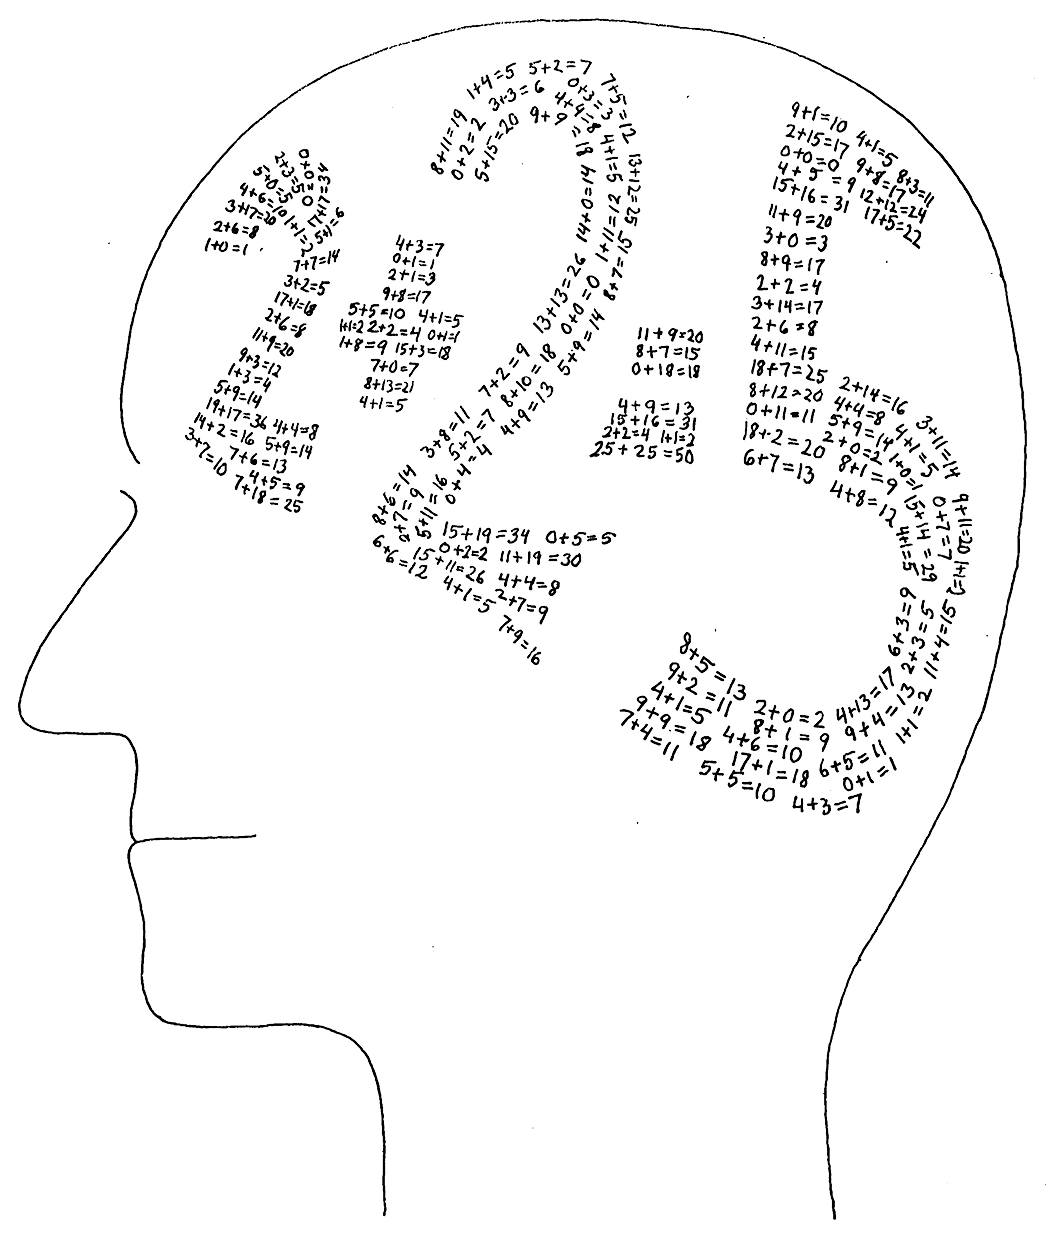
\includegraphics{img_109.png}
\caption[大脑的低层与高层之间的冲突。]
  {大脑是理性的,而心智则可能不是。[作者绘]}
\end{figure}

这种观点——在先前讨论各种各样的问题时曾多次提到——其实就是说:意义可以存在于符号操作系统的两个或多个不同的层次上,而且与意义一道,正确性与错误性能在所有这些层次上存在。意义在一个给定层次上的出现,取决于现实世界是否是以一种同构(还是较为松散的)的形式在这个层次上得到反映。所以,神经元总是正确地执行加法(其实,是比加法复杂得多的计算),这一事实完全不能担保它们的机制所支持的最高层结论是正确的。即便大脑的最高层忙于证明布尔佛教的公案,或者忙于冥想禅宗代数的定理,它的神经元却仍在合理地行动着。同理,大脑中感受美的经验的高层符号过程,其底层是完全理性的,那里发生着完美无缺的行动。任何非理性的东西,如果存在,就是在较高的层次上,而且是低层事件的旁效现象一个后果而已。

为了从另一个角度来看这个问题,我们来假定你正难以做出决定,不知是该要一盘茄汁鳜鱼还是黄连汁鳜鱼。这是不是就蕴涵着你的神经元细胞也受到阻碍,而难以决定它们是否发射呢?当然不是。你的鳜鱼混乱是一个高层王国的事件,以很有组织的方式依赖于数以千计的神经元的总体的有效发射。这多少有点讽刺,然而只要想一想,就会觉得是完全明白的。尽管如此,断定有关心智和计算机的几乎全部的混乱都来源于这种基本的层次混乱,大概是十分公平合理的。

没有什么理由使人相信,一台计算机中运转得完美无缺的硬件不可能支持那些体现诸如混乱、遗忘以及美感这类复杂事件的高层符号行为。这将需要大量的子系统按照一种复杂的“逻辑”相互作用。表面的行为可能表现为理性或非理性,然而暗地里则应该是可靠的逻辑硬件的工作。

\section{再驳卢卡斯}

这种层次区别倒顺便给我们提供了与卢卡斯辩论的某种新武器。卢卡斯的论证建立在“哥德尔定理按其定义可用于机器”这样一种思想之上。事实上,卢卡斯极力宣称:

\begin{quote}
哥德尔定理必定适用于控制论机器,因为作为机器的本质特征,机器该是形式系统的一个具体特例。\note{安德森编卢卡斯文,第44页。}
\end{quote}

如我们已经看到的,在硬件层次上这是真的——然而由于或许还存在更高的层次,所以这不是关于这个论题的最后断语。卢卡斯强调说,在他所讨论的模拟意识的机器里,只有一个层次上发生了符号操作。例如分离规则(在他的文章中叫“假言推理”)就要做成硬件,并将成为这样一台机器的一个不可改变的特性。他更进一步地宣称,如果假言推理不是该机器系统的永远不变的栋梁,而是可以偶然撇开的,那么:

\begin{quote}
该系统将不再是一个形式的逻辑系统,而且该机器将胜任心智的模型这个角色。\note{安德森编卢卡斯文,第54页。}
\end{quote}

在人工智能研究中正在开发的很多程序与那些生成数论真理的程序——一些具有不变的推导规则和固定的公理集合的程序——没有多少共同之处,而且它们当然是有意做成“心智模型”的。在它们的顶层——“非形式”层次——可能有一些意象的操作、类比的形式、念头的遗忘、概念的混淆以及差别的抹杀等等。不过,这并不与下述事实相矛盾:它们就像大脑依赖其神经元的正确行动一样,依赖于支持它们的硬件的正确行动。所以,人工智能程序依然是“形式系统的具体实例”——不过他们不是能应用卢卡斯所曲解了的哥德尔证明的那种机器。卢卡斯的论证只适用于它们的底层,可是它们的智能——不论高低——并不依赖那个底层。

我们还可以从另一个角度考察卢卡斯对“心智过程必须怎样在计算机程序内部表示”这个问题的那个过于简单的看法。在讨论一致性问题时,他写到:

\begin{quote}
如果我们实际是些不一致的机器,我们就应满足于这种不一致性,从而痛痛快快地肯定一对矛盾的两个方面。更进一步,我们该是可以随便讲任何事情——但我们没有这样。容易说明,在一个不一致的形式系统内,一切都是可证的。\note{安德森编卢卡斯文,第53页。}
\end{quote}

最后这句话表明,卢卡斯假定了命题演算一定得包含在任何一个能做推理的形式系统之中。具体地说,他是在考虑命题演算的定理$<<"P"∧~"P">→"Q">$。显然,他错误地认为这是机械化推理的一条必不可少的要素。无论如何,要是说像命题推理这样的逻辑思维过程是一个人工智能程序的一般智力的结果,而不是预先程序化了的东西,是完全有可能的。这恰是在人类身上发生的事情!没有什么特别的理由该假定狭义命题演算——连同它们所必需的刻板规则,以及有关一致性的呆笨的定义——都得要出现在这样一个程序之中。

\section{人工智能的一个基点}

我们可以把这一通闲扯都归结到层次的区分。在离开这个话题之前,我们给出丘奇—图灵论题的一个最强的——也是最后的——形式:

\begin{thm}[2\ccwd]{丘奇—图灵论题,人工智能形式}
任何种类的心智过程都可以用一个计算机程序来模拟,而该程序的基础语言与FlooP一样强,也就是说全体部分递归函数都能用这种语言程序化。
\end{thm}

还需要指出的是,实际上很多人工智能研究者信奉的是与丘奇—图灵论题密切相关的另一个信条,我把它叫做人工智能论题,叙述如下:

\begin{block}
人工智能论题:随着智能机的发展,它的基础机制会逐渐收敛于人类智能的基础机制。
\end{block}

换句话说,一切智能都只是同一主题的各种变奏。为了创造真正的智能,人工智能工作者如果想要使他们的机器达到我们所具有的能力,他们就得坚持深入那些较低的层次,使之越来越接近大脑的机制。

\section{丘奇定理}

现在,让我们回过头来看螃蟹,再看看他的定理资格判定过程(伪装成一种判定音乐美的过滤器)是否与现实世界相容这一问题。实际上,根据对话中提到的事实,我们没有办法推定螃蟹的才智是不是一种分清定理和非定理的能力,或者换个说法,分清真陈述和假陈述的能力。当然,在很多情形下这是一回事,不过\emph{哥德尔定理}表明这并不总是一回事。但是,这没有关系:如果我们相信丘奇—图灵论题的人工智能形式,那么这两种说法都不可能是真的。在任何强如TNT的形式系统中都不可能有判定定理的过程——这个命题叫\emph{丘奇定理}。没有一个判定数论真理的过程——如果这种真理存在的话。读者在看过TNT的全部分叉现象之后,很可能会怀疑这种存在性——这样一个命题可以很快地从\emph{塔斯基定理}(发表于1933年。实际上其思想在此之前就早已为塔斯基所知)推出。

这两个极为重要的元数学结果的证明是很相似的。它们都可以很快地从一个自指结构中得到。我们先来考虑TNT定理的判定过程。如果存在一个统一的方法使人们可以判定一个给定的公式X究竟应归入“定理”类还是“非定理”类,那么,根据丘奇—图灵论题(标准形式),就该有一个有终止的FlooP程序(一般递归函数),当给出公式X的哥德尔数作为输入时,该程序能给出与上述方法相同的判定。其关键步骤在于(读者应该还记得):能用一个有终止的FlooP程序检测的任何一种性质在TNT中都有一个体现。这意味着“是TNT定理”这条性质能在TNT内部体现(与仅仅表示是不同的)。然而,如我们马上就能看到的那样,这会使我们陷入困境,因为如果“是定理”是一个可体现的属性,那么哥德尔公式G就会是与说谎者悖论同样可怕了。

这全是因为G在说:“G不是TNT定理”。假如G是定理,那么由于“是定理”按假定应可体现,所以断言“G是定理”的那个TNT公式应当是TNT定理。而这个公式就是$~\moG$,即G的否定。所以TNT就不一致了。另一方面,假如G不是定理,那么根据假设的定理资格的可体现性,断言“G不是定理”的那个公式就应是TNT定理。然而这个公式就是G,所以我们仍得到悖论。与前面的情形不同,这里根本无法消除这个悖论。问题之所以出现,就是由假定“是定理”这一性质可由某个TNT公式体现。因而,我们就必须追溯回去,摒弃这个假设。这就迫使我们得出:没有一个FlooP程序能分清定理的哥德尔数和非定理的哥德尔数。最后,如果我们接受丘奇—图灵论题的人工智能形式,那我们就得进一步地回溯,得出:无论如何都不会有什么方法能使人类可靠地分清定理和非定理——这也包括基于美感的判断。那些只同意丘奇—图灵论题的大众过程形式的人,可能仍然认为螃蟹的成就是可能的。不过,在丘奇—图灵论题的所有各种形式当中,这一个也许是最难得到支持的。

\section{塔斯基定理}

现在我们接着看塔斯基的结果。塔斯基问,是否可以有一种在TNT中体现数论真理概念的方法。我们已然看到“是定理”这个性质是可表示的(尽管不是可体现的)。塔斯基则对于有关真理概念的类似问题产生了兴趣。尤其是,他希望确定是否会有一个只含一个自由变元$a$的TNT公式,它可以翻译成:

\begin{block}
“哥德尔数为$a$的公式表示一条真理”。
\end{block}

像塔斯基那样,我们先来假定有这样一个公式——把它缩写成$"TRUE"\{a\}$。然后,所要做的事情就是使用对角线方法制造一个句子,它对自己下断语,说自己不是真的。我们完全照搬哥德尔的方法,从一个“服”号串入手:
\[
\exists a:<~"TRUE"\{a\}∧"ARITHMOQUINE"\{a'',a\}>
\]
把这个“服”号串的哥德尔数记作$t$,然后就算术㧟摁它,从而得到塔斯基公式T:
\[
\exists a:<~"TRUE"\{a\}∧"ARITHMOQUINE"\{
\underbrace{SSS\cdots SSS}_{\text{$t$个$S$}}0/a'',a\}>
\]
如果解释一下,它是在说:

\begin{block}
“$t$的算术㧟摁化是个假陈述的哥德尔数。”
\end{block}
可是由于$t$的算术㧟摁化是T自身的哥德尔数,所以塔斯基公式T恰好在TNT中重现了说谎者悖论,它在说自己:“我是假话”。当然,这就导致了结论:它既真又假(或既不真又不假)。于是又产生了一个令人感兴趣的问题:说谎者悖论的出现有什么不好?这有什么要紧的吗?毕竟汉语中已经有了这个悖论,而中国语言并没有因此就灰飞烟灭。

\section{那个被赞美的螃蟹是不可能存在的}

其答案就在于:别忘了这里牵涉到了意义的两个层次。一个层次是我们刚才用过的,而另一个层次则是作为一个数论陈述。如果塔斯基公式T真的存在,那它就是一个同时既真又假的论及自然数的陈述!难就难在这里,尽管对于汉语来说,说谎者悖论总能因其话题(它自己的真理性)过于抽象而清除掉,可这一个却不然,因为它变成了一个严格的数论陈述!如果我们相信这是一种荒唐可笑的事态,那就只好丢掉TRUE{a}是存在的这一假设。就是说没有一种方法能在TNT内部表示真理的概念。应当看到,这个结果就使得“是真理”成为比“是定理”更难以捉摸的性质,因为“是定理”还是可表示的。按照前面(涉及丘奇—图灵论题的人工智能形式)谈过的回溯推理,我们得到结论:

\begin{block}
“螃蟹的心智辨认起真理来,一点也不比辨认TNT定理更强。”
\end{block}
因为前一种辨认违背\emph{塔斯基—丘奇—图灵定理}(“不存在确认算术真理的判定过程”),而后者则违背了\emph{丘奇定理}。

\section{形式的两种类型}

当把“形式”这个词用于各式各样形状复杂的结构时,想想它的意义是很有意思的。例如,当我们观赏一幅画并感到美时,引起我们反应的是什么?是视网膜上的点和线的“形式”吗?显然一定是的,因为它就是如此进入我们头脑的分析机制的——不过这一处理过程的复杂性使我们感到并不只是看到了一个二维的表面,我们在对这幅画的某种内在意义——某种莫名其妙地陷入了二维的那个多维对象——产生共鸣。这里重要的是“意义”这个词。我们的心智有一些接受二维模型的解释机制,然后再从中“抽”出高维概念,这些高维概念复杂得我们无法有意识地对之进行描述。其实,我们对音乐的反应也是一样。

主观感觉是,抽出内在意义的机制完全不同于检验有还是没有某种特定性质(比如一个符号串是否良构)的判定过程。也许这是因为内在意义过一段时间以后会泄露出更多的东西。我们永远不可能像对良构性那样有把握地确定什么时候才算大功告成了。

这提示了一种区分,在我们所分析的模式中,对“形式”的两种含义可以作个区分。首先,有一些性质,如良构性,它们可以用预知有终止的检验来检查,比如用BlooP程序。我把这些性质叫做形式的句法性质。直观上可以察觉到,形式的句法方面比较接近于表面,因而并不能激发多维认知结构的创造。

作为对照,形式的语义方面是不能在预定时间期限内检验的:它仍需要无尽头的检验。如我们已经看到的,检验TNT符号串是不是定理这种情形就是如此。你无法把某个标准的检验法用于一个符号串,以辨认出它是否是一条定理。不知什么原因,“涉及到了意义”这一事实,与弄清一个符号串是否是TNT定理的难度,是密切相关的。从本质上说,抽出一个符号串的意义的行为,涉及到建立它与其它所有符号串之间相关联时的全部意味,而这当然就导致一个无尽头的征途。所以,语义性质就与无终止的搜索联系在一起了。因为,在一个很重要的意义上,一个客体的意义并不局限于该客体自身之内。这自然并不是要说在时间终结之前就不可能理解任何客体的意义。因为,随着时间的流逝,越来越多的意义变明朗了。但是,不论过多久,也不可能发现其意义的所有方面。

\section{意义来自认知结构间的联系}

让我们从符号串转向乐曲,变个花样看看。如果你愿意的话,仍可把每一处提到乐曲的地方都换成“符号串”。这种讨论必然是一般性的,只不过我觉得还是谈音乐更容易使人理解其韵味。乐曲的意义有一种少见的两重性:一方面,凭借着它与世界上其它很多事物的关系,似乎要向四周蔓延——而另一方面,一段乐曲的意义显然源自音乐本身,所以它必定能定位于音乐内部的某个地方。

考虑解释机制可以摆脱这种窘境。所谓解释机制就是抽出意义的那种机制(这里说的解释机制并不是指乐曲的演奏者,而是指欣赏该曲时从中得出意义的那位听众的心理机制)。当第一次听到某首乐曲时,解释机制会发现它的意义的很多重要方面。这似乎证明了意义寓于乐曲自身之内、并可从中直接读出这样一种观念,不过这只是问题的一部分。音乐解释机制是通过建立一个多维的认知结构——该乐曲的一个心智表示——而工作的。这个多维认知结构努力寻找与那些为以前的经验编码的多维心智结构之间的联系,借此同早就存在的信息结合起来。随着这个过程的进行,整个意义就逐渐显露出来了。事实上,当一个人感到他已经悟透一段乐曲的核心意义时,可能若干年的时间已经过去了。这似乎又有利于相反的观点:音乐的意义向四方延伸,解释机制的作用就是逐步收集它。

真理毋庸置疑是位于这两者之间的某个地方:无论音乐的意义还是语言的意义,在某种程度上都是可定位的,在某种程度上又都是向四方延伸的。用第六章的话来说,我们可以说乐曲和文章都既是显明意义的触发器,又是运载者。可以通过一块刻有铭文的古碑的例子,来给意义的这种两重论作个生动的说明:碑文的意义部分地贮存在世界各地的图书馆和学者们的大脑之内,但它显然也隐含在古碑自身之内。

于是,要刻划“句法”性质和“语义”性质(在刚刚提到那种意义下)之间的差别就还有一条路子,即:句法性质毫不含糊地存在于所考虑的客体之内,而语义性质则依赖于它与潜在地无穷多的客体类之间的关系,因而不是完全可以定位的。原则上说,句法性质中没有什么秘密或隐藏的东西,然而这种隐蔽性却是语义性质的本质。这就是我区别视觉形式的“句法”方面和“语义”方面的理由。

\section{美、真与形式}

美又怎么样呢?按照上面的思想,它当然不是句法性质。那么它能是语义性质吗?比方说,美是某幅具体的画所具有的性质吗?让我们干脆就限于考虑一个观察者。每个人都有过这样的经验:这个时候觉得某个东西很美,那个时候又会觉得它很丑——而其它时候又可能觉得它很平常。那么,美是不是一个随时间变化的属性呢?但是倒过来也可以说,随时间变化的是那位观察者。那么,当确定了一个在特定的时间观赏一幅特定的画的特定的人之后,是否就有理由断定美是一种确确实实的、或者存在或者不存在的性质呢?还是说,有关美的问题仍然还有某些定义不清的、不可捉摸的东西?

随着环境的变化,在每个人心里都可能会引发解释器的不同层次。这些形形色色的解释器抽出不同的意义,建立不同的联系,并一般地对所有深入的方面给出不同的评估。所以,看起来,美这个概念极难把握。正因为如此,我才在《的确该赞美螃蟹》中把美与真联系在一起,我们已经看到,“真”乃是整个元数学中最不好捉摸的概念之一。

\section{说谎者悖论的神经基质}

我打算以关于真理的那个中心问题——即说谎者悖论——的某些想法,作为本章的结尾。我认为,塔斯基在TNT内部对说谎者悖论的复制,指出了深入理解汉语中的说谎者悖论的一个途径。塔斯基所发现的东西是:该悖论的塔斯基形式有两个不同层次。在一个层次上,它是谈论自身的句子,如果它假,那就会真,如果它真,就又会假。在另一个层次——我喜欢把它叫作算术基质——上,它是一个谈论整数的句子,它为真当且仅当它为假。

这样一来,由于某种原因,这后一种说法就比前一种更为令人费解。由于前一种说法的自指性,有人就干脆贬斥为“没有意义”。但你却不能这样贬斥一个谈论整数的悖论陈述,谈论整数的陈述根本不能既真又假。

我的感觉是:塔斯基对说谎者悖论的转换指导了我们去寻找该悖论汉语形式的基质。在其算术形式中,高层的意义建立在低层的算术层次之上。也许与之类似,我们见到的那个自指句子(“本句子是假的”)只是一个双层次统一体的顶层。那么较低的层次又是什么呢?支持语言的结构又是什么呢?是大脑。所以必须给说谎者悖论找一个神经基质——一个较低的、由互相冲突的物理事件——也就是按其性质而言不能同时出现的事件——组成的层次。如果这种物理基质存在,那么我们之所以无法理清说谎者句子的来龙去脉,就是由于我们的大脑在试图作一件力所不及的事情。

那么,这些互相冲突的物理事件的实质又是什么呢?也许当你听到说谎者句子时,你的大脑就建立了该句子的一种“编码”——相互作用的符号的一种内部布局。然后,它就试图把句子归结为“真”、“假”两类。这种分类行为必定迫使某些符号按一种特殊的方式发生相互作用(也许遇到任何一个句子时都会发生这种过程)。如果碰巧这种分类行动会从物理上搞乱该句子的编码动作——一种轻易不会发生的事情——那就算碰上麻烦了,因为它相当于试图要一台唱机播放毁坏它自己的唱片。我们用物理术语而不是用神经学的术语描述了这种冲突。如果这种分析到现在为止还是有效的,那么当我们了解了一些大脑中来自神经元及其发射的“符号”建构,又了解了一些给句子编码的方式时,余下的讨论就可以继续下去了。

说谎者悖论的神经基质的这幅草图(至少对我)暗示了:说谎者悖论的汉语形式的这种解决,很可能类似于该悖论的塔斯基形式的解决。这种解决包括放弃“大脑总是能够为真理概念提供一个完全精确的描写”这样一种观念。这种解决的新颖性,在于它暗示着给出真理的全面模型是不可能的,而这是由于一个来自物理方面的理由,即:做这样一个模型从物理上需要在一个大脑中出现不相容的两个事件。
